 
\section{Problem 1}
\label{part1}
\begin{verbatim}
Download the 1000 URIs from assignment #2. ``curl'',``wget'', or
``lynx'' are all good candidate programs to use.  We want just the
raw HTML, not the images, stylesheets, etc.

from the command line:

% curl http://www.cnn.com/ > www.cnn.com

% wget -O www.cnn.com http://www.cnn.com/

% lynx -source http://www.cnn.com/ > www.cnn.com

``www.cnn.com'' is just an example output file name, keep in mind
that the shell will not like some of the characters that can occur
in URIs (e.g., ``?'', ``&'').  You might want to hash the URIs, like:

% echo -n ``http://www.cs.odu.edu/show_features.shtml?72'' | md5
41d5f125d13b4bb554e6e31b6b591eeb

(``md5sum'' on some machines; note the ``-n'' in echo -- this removes
the trailing newline.) 

Now use a tool to remove (most) of the HTML markup.  ``lynx'' will
do a fair job:

% lynx -dump -force_html www.cnn.com > www.cnn.com.processed

Use another (better) tool if you know of one.  Keep both files 
for each URI (i.e., raw HTML and processed).
\end{verbatim}

\subsection{Solution}

\begin{enumerate}
\item I started the 1st question by running a sample URI with curl command syntax as given in the question.  This created a new file in my directory with html content of the URI that I have mentioned.
\item So I got to know by executing the curl command I will be getting raw data file of the URI.
\item Now the next important point is naming the output files. If we name the output files with URI names,then i will be getting error at one point because it does not accept special characters.
\item This issue can be resolved by creating a hash code which is unique for each URI. I used hashlib library to convert URIs to respective hash codes. 
\item Now I have named the file as Raw or processed followed by unique number for each URI followed by the hash code. I add unique number so that it would be useful for me to get URI back from the hash code in future.
\item The same process should be repeated with lynx command(given in question) to get processed file which eliminates all the html content and gives only data.
\item I have written a loop which runs 1000 times and each time it takes a URI and generates a raw file and a processed file. Therefore at the end I will be getting 1000 raw files and 1000 processed files.
\item The code for this program is shown below. Figure 1 and Figure 2 shows a sample Raw file and sample processed file. Figure 3 and Figure 4 shows list of raw and processed files created. 
\end{enumerate}
\newpage
\subsection{Code Listing}
Here is the Python program for acquiring raw and processed data files for each URI. 


\lstinputlisting[language=Python,breaklines = true,frame=single,caption={Python program for acquiring raw and processed data files for each URI}, label=lst:q1-1,captionpos=b,numbers=left,showspaces=false,showstringspaces=false,basicstyle=\footnotesize]{raw_and_processed_data.py}
\newpage
\subsection{Results}


\subsubsection{Sample Raw File}
\begin{figure}[ht]    
    \begin{center}
        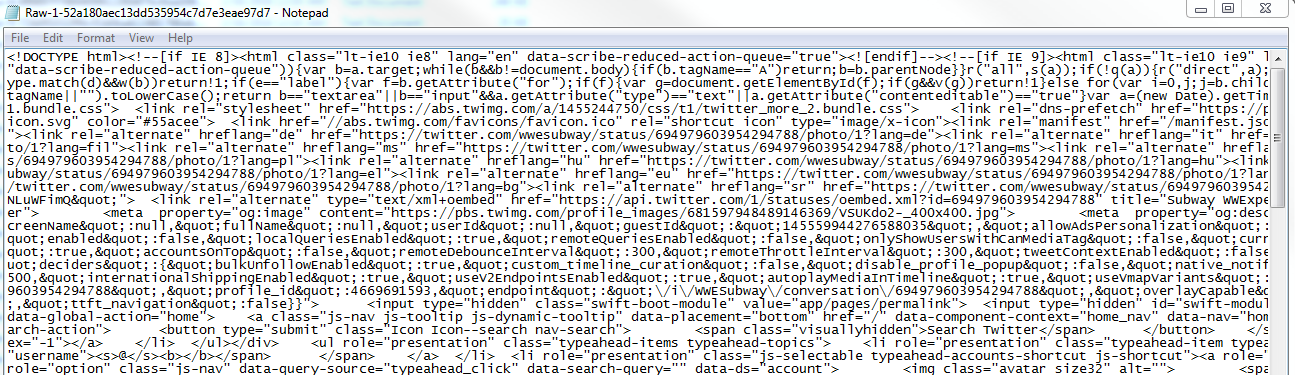
\includegraphics[scale=0.5]{Raw_sample.png}
        \caption{Sample Raw File}
        \label{Sample Raw File}
    \end{center}
\end{figure}

\subsubsection{Sample Processed File}
\begin{figure}[ht]    
    \begin{center}
        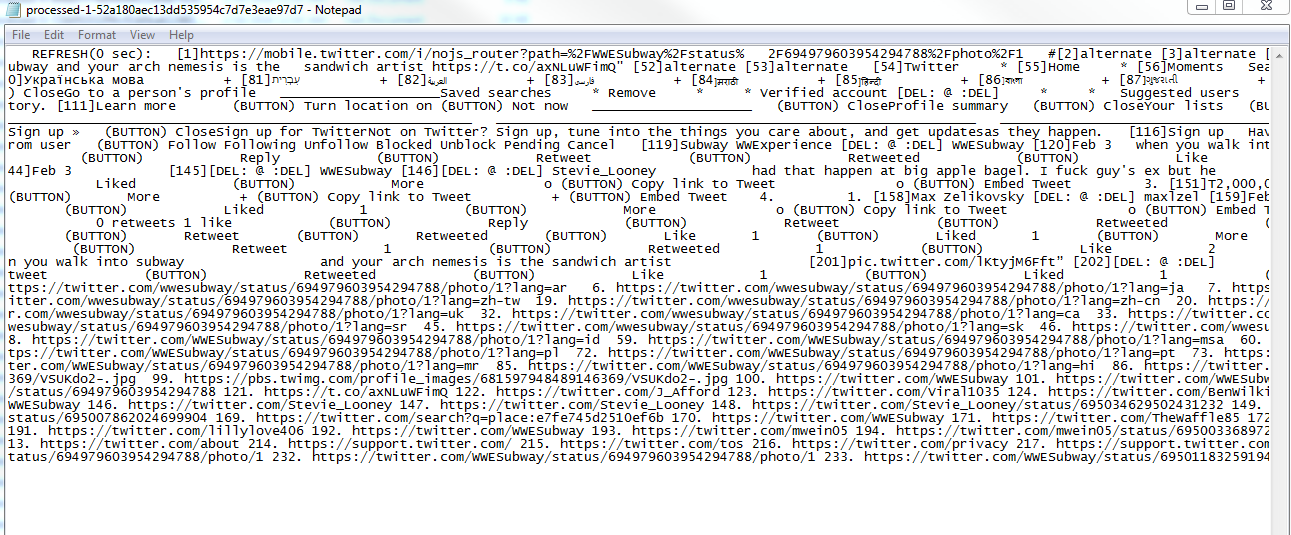
\includegraphics[scale=0.5]{processed_sample.png}
        \caption{Sample Processed File}
        \label{Sample Processed File}
    \end{center}
\end{figure}
\newpage
\subsubsection{Sample Collection of Raw files}
\begin{figure}[ht]    
    \begin{center}
        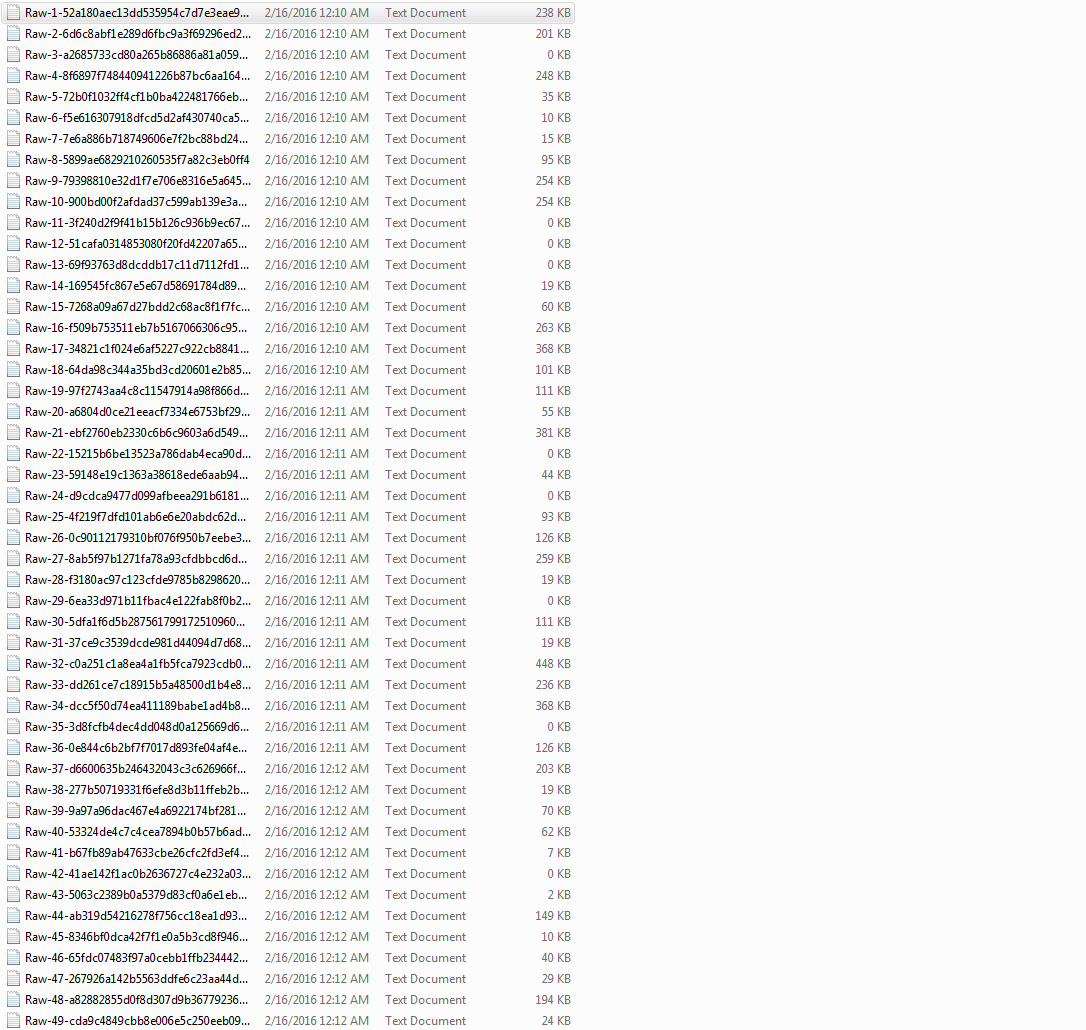
\includegraphics[scale=0.6]{raw_coll.png}
        \caption{Sample Collection of Raw files}
        \label{Sample Collection of Raw files}
    \end{center}
\end{figure}
\newpage
\subsubsection{Sample Collection of Processed files}
\begin{figure}[ht]    
    \begin{center}
        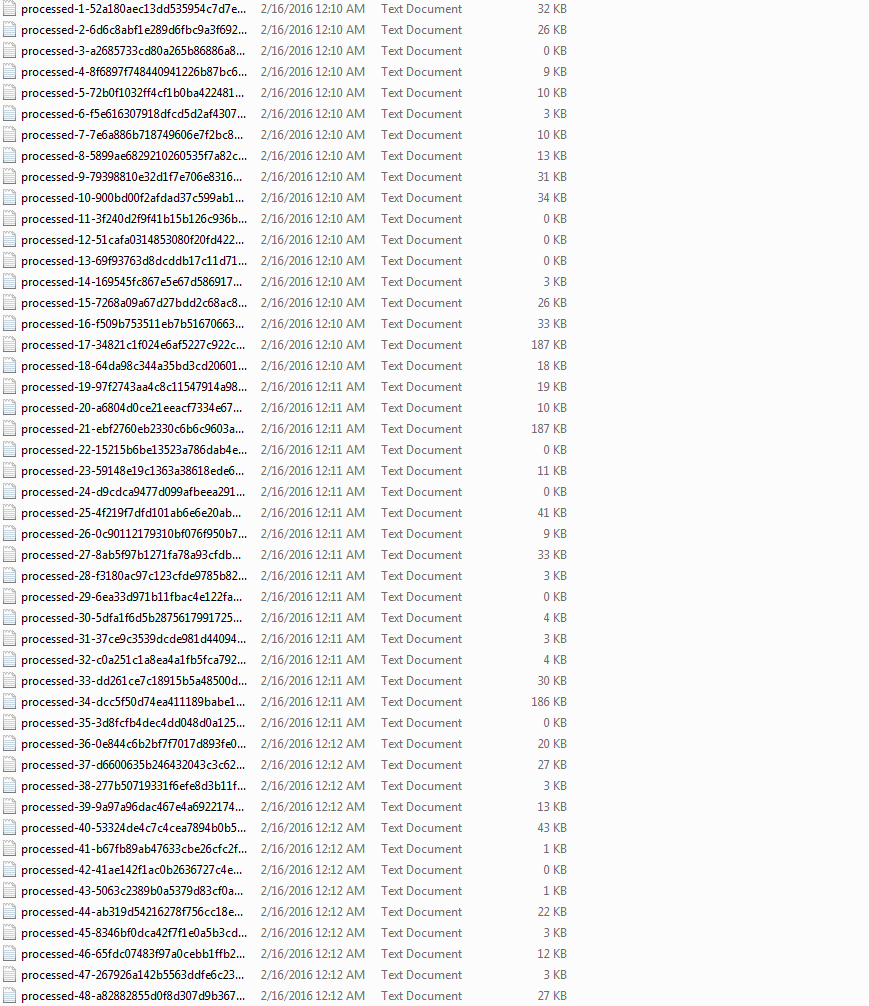
\includegraphics[scale=0.6]{process_coll.png}
        \caption{Sample Collection of Processed files}
        \label{Sample Collection of Processed files}
    \end{center}
\end{figure}
\newpage
